\def\year{2015}
\documentclass[letterpaper]{article}
\usepackage{aaai}
\usepackage{graphicx}
\usepackage{algorithm}
\usepackage{algpseudocode}
\usepackage{amsmath}
\usepackage{amssymb}
\usepackage{amsthm}
\usepackage{etoolbox}
\usepackage{color}
\usepackage{changepage}
\usepackage{csquotes}
\usepackage{tabularx,booktabs,multirow}
\usepackage{longtable}
\usepackage{framed}

\pdfinfo{
/Title (Learning Constraints and Optimization Criteria)
/Author (Samuel Kolb)}
\setcounter{secnumdepth}{0}  

\graphicspath{{Graphics/}}

\newcommand{\sym}[1]{\ensuremath{\mathcal{#1}}}
\newcommand{\svm}{SVM$^{rank}$}

\newtheorem{definition}{Definition}[section]
\newtheorem{question}{Question}
\AfterEndEnvironment{definition}{\noindent\ignorespaces}

\theoremstyle{definition}
\newtheorem{example}{Example}
\newtheorem{experiment}{Experiment}[question]
\newtheorem{observation}{Observation}[question]

\setlength{\tabcolsep}{6pt}

\begin{document}

\title{Learning Constraints and Optimization Criteria}
\author{
  Samuel Kolb\\
  KULeuven, Leuven, Belgium\\
  samuel.kolb@cs.kuleuven.be
}

\maketitle

\begin{abstract}
This paper presents a system that is able to automatically learn both constraints from examples and optimization criteria from rankings.
Both hard and soft constraints can be learned and constraints are represented as first order logical clauses.
Choosing such clauses as representations enables the use of ILP techniques such as clausal discovery.
In this research, optimization criteria are represented as weighted clauses.
For all examples, the clause learning system could find the essential constraints efficiently.
The learning system for optimization criteria is shown to achieve accurate results and can learn criteria that identify the correct optimal solution even for few examples and noisy rankings.
Finally, a procedure is outlined that allows weighted first order logic clauses to be used for optimization.
\end{abstract}

\section{Introduction}
This research tackles the learning of constraints and optimization criteria.
Non-experts often experience difficulties when modeling a problem using constraints \cite{Wallace:PrinciplesCP}.
The first goal of this research is to automate the step of modeling a problem, in order to, amongst others, make constraint solving more accessible.
In this approach a few examples of what a user considers valid solutions are used by a computer system to find constraints.
These constraints can then be used by an existing constraint solver.

Constraints are represented as logical clauses.
This representation allows for the use of techniques from the field of Inductive Logic Programming (ILP).
Specifically, a new implementation of the Clausal Discovery algorithm \cite{DeRaedt:ClausalDiscovery} is used.
Research on constraint learning is often done independent of ILP.
By exploiting the parallels between both fields, this research follows the same approach as \cite{Lallouet:LearningCP}.

Hard constraints are used to distinguish solutions to a problem.
So called soft constraints can be used to express properties which do not have to be fulfilled by every solution.
Soft constraints are assigned weights that express their importance.
Such weighted soft constraints can be used as optimization criteria.
Optimal solutions are found by maximizing the sum of the weights of soft constraints that are fulfilled by a solution.

The second goal of this research is to learn from user preference and to formulate corresponding optimization criteria.
By using rankings over a few examples, weighted soft constraints can be found.
Both the learning of constraints as well as the learning of optimization criteria aim to bridge the gap between problems and their formal representation.

The use of weighted soft constraints is inspired by the research of \cite{campigotto2011active}, amongst others.
Their work examines attempts to obtain similar results in an interactive context for propositional constraints.
In this research, first-order logical clauses will be used.

The weighted clauses cannot be directly used by a constraint solver.
Therefore, an approach is outlined that describes how these constraints can be used in an existing solver to obtain an optimal solution in practice.

This research has been conducted during the course of my masters thesis~\cite{kolb2015thesis}.
\section{Background}
In this section a brief overview of the important concepts and relevant literature will be provided.

\subsection{Clauses}
First-order logical clauses consist of a disjunction of literals.
Literals are defined as being either an atom or a negated atom.
Clauses are often expressed using a body and a head: $\mathit{head} \leftarrow \mathit{body}$.
All literals containing a negation are grouped in the body and the other literals form the head of the clause.
For example, $\lnot a_1 \lor \lnot a_2 \lor a_3 \lor a_4$ corresponds to the clause $a_3, a_4 \leftarrow a_1, a_2$.

Atoms are logical concepts that can be assigned a truth value.
In this paper, atoms will be restricted to either the symbols $\mathit{true}$ or $\mathit{false}$ or a predicate.
Predicates consist of a predicate symbol and a set of terms.
Terms are either constants or variables and describe objects in a domain.
Predicates express relations between these objects: $\mathit{symbol}(\mathit{term_1}, ... \mathit{term_n})$.
Clauses are universally quantified and will, in this research, only contain variables.

\subsection{Learning constraints}
Constraint learning is a hard problem.
The search space of constraints is typically very large.
Furthermore, there are usually only a few examples to learn from, unlike in typical machine learning problems.

Different systems attempt to learn constraints using different methods.
The problem of having little examples can be alleviated by interactively generating data.
Both the systems Conacq2 \cite{bessiere2007query} en QuAcq \cite{bessiere2013constraint} generate (partial) examples and query the user about their validity.

ModelSeeker \cite{Beldiceanu:ModelSeeker} attempts to structure the problem variables in different ways.
The system then tests for different global constraints whether they hold within this structure.
This approach allows for constraint learning from a few examples.

As mentioned earlier, the research of \cite{Lallouet:LearningCP} already tried to use ILP techniques to learn constraints.
In their approach, the search space of constraints is explored in a bidirectional manner, primarily using negative examples.


\subsection{Clausal Discovery}
The clausal discovery algorithm proposed by \cite{DeRaedt:ClausalDiscovery} attempts to learn first order logic clauses from positive examples.
Using a refinement operator, the search space is traversed by incrementally generalizing clauses until they cover all examples, starting from the empty clause~($\square$).
The result set consists of the most specific clauses covering all examples.
This research uses the clausal discovery algorithm on a high level but provides a very different implementation than the original clausal discovery engine.

\subsection{Logic Solver}
The logic system IDP \cite{de2013prototype,wittocx2008idp} is used to calculate whether examples satisfy clauses and is used as a theorem prover.
It supports an extension of first order logic ($FO(\cdot)$) and can also be used to generate new solutions.
Background knowledge is given as an IDP theory.

\subsection{Optimization}
The Boolean Satisfiability Problem (SAT) attempts to determine whether a propositional formula can be satisfied.
Formulas can be rewritten into a special form called the conjunctive normal form (CNF), which consists of a conjunction of clauses (disjunctions).
An extension of this problem is the Maximum Satisfiability Problem (MAX-SAT).
In MAX-SAT the amount of satisfied clauses is maximized.
By assigning positive integer weights to clauses and maximizing the sum of the weights of satisfied clauses, one obtains the weighted MAX-SAT problem.
The work by \cite{campigotto2011active} attempts to learn propositional formulas en weights automatically.
Inspired by their results, this research tries to learn first-order logic optimization criteria.
The resulting optimization problem can be seen as an extension of weighted MAX-SAT in which the clauses are in first-order logic.

\section{Problem Statement}
This research has two main objectives: learning constraints and learning optimization criteria.
The system designed to solve these problems attempts to simplify the process of generating formal representations.
Therefore, it should be easy to use and take into account what kind of information a user can provide.

\begin{framed}
  \noindent
  \begin{minipage}{\textwidth}
    \paragraph*{Goal 1}
    Given a set of examples and a limit $t$, the goal of the constraint learning system is to find maximally specific clauses that are satisfied by at least $t$ of the given examples.
  \end{minipage}
\end{framed}

Examples describe specific solutions.
They contain a set of objects and exhaustively describe all relations (predicates) that hold on these objects.
The learned clauses are independent of the specific objects within the examples and contain only variables.

\begin{example}
  Consider sudoku as an example of a problem where hard constraints are to be found.
  Given one or more solved sudokus, the learning system has to identify the rules of the game.
  Since the learned clauses only contain universally quantified variables, for example $4 \times 4$ sudokus could be used to find constraints.
  The learned constraints are independent of the size of the sudoku and can also be used to solve $9 \times 9$ sudokus, for example.

  In some problems, one is interested in regularities that  often but not always occur.
  An example would be regularities in certain types of buildings.
  While certain regularities would occur in many buildings, there are often exceptions and different styles.
  In this case, one could attempt to find constraints on the structure of the floor plans that are satisfied by a given amount of examples.
\end{example}

\begin{framed}
  \noindent
  \begin{minipage}{\textwidth}
    \paragraph*{Goal 2}
    Given a set of examples and a set of partial rankings over these examples, the goal of the optimization system is to learn soft constraints and weights such that the order described by these optimization criteria maximally corresponds with the given rankings.
  \end{minipage}
\end{framed}

The soft constraints consist of clauses that are satisfied by some of the examples.
Rankings are partial orders over the examples: $e_x = e_y > ... > e_a = e_b$.
The weighted clauses can be used to calculate a score for every example
\begin{eqnarray*}
  \sum\limits_{\mathit{weight}, \mathit{c}} \mathit{weight} \cdot v_{c}
\end{eqnarray*}
With $v_c = 1$ if the clause $c$ is satisfied by the example and $v_c = 0$ if $c$ is not satisfied.
These scores allow for a total order over all examples to be defined. 

\begin{example}
  Consider the scenario of moving to a new city.
  Multiple job offers are available, different accommodations are to be considered and there are different schools in the city.
  Learning weighted soft constraints can make user preferences explicit.
  For example, it could be desirable that the school is in a low crime area or that the locations of the school and work place are close.
\end{example}

A third goal of this research is to show how these constraints and especially the optimization criteria can be used in practice to find an optimal solution.

\section{Approach}
\begin{figure}

  \centering
    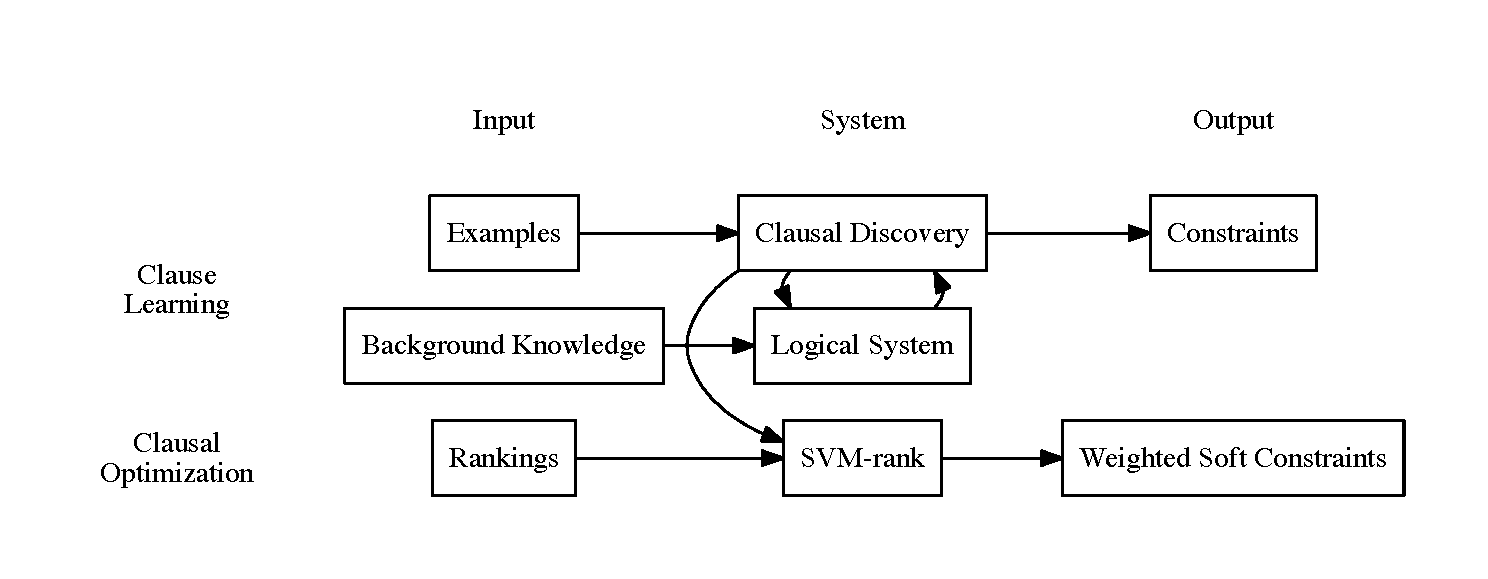
\includegraphics[width=0.8\linewidth]{ApproachOverview.pdf}
  \caption{Overview approach}
  \label{fig:struktuur}

\end{figure}

In this research, both constraint learning and learning optimization criteria were implemented.
An overview is presented in figure~\ref{fig:struktuur}.
Clauses are learned using examples.
To find weighted clauses, first the constraint learning system is used to find soft constraints.
Then the weights for these soft constraints are determined based on the rankings.
In order to determine the weights, the \svm system is used.

\subsection{Input}
The input consists of examples and definitions.
Every example contains a set of constants that are part of the model and an exhaustive list of the relations that hold on these constants.
Definitions describe either typing information or predicate definitions.
Typing information relates directly to the problem domain, improves the accuracy and efficiency of the learned clauses, and is usually easy to provide for the user.
Predicate definitions describe the types of the terms occurring in a predicate.
Two special types of predicates are allowed: calculated predicates and symmetric predicates.
Calculated predicates are not listed in examples, instead background knowledge is used to generate them.
Symmetric predicates are predicates for which the order of the terms does not matter.
If optimization criteria are to be learned, a set of rankings over the given examples is also provided.

\begin{example}
  Imagine a problem that describes humans with a type \textit{human} and predicates human(\textit{human}), male(\textit{human}) and female(\textit{human}).
  An example could contain the constants S and A, both of type \textit{human}, and the relations: human(S), human(A), male(S), female(A).
  Clauses to be learned would be: human(x) $\leftarrow$ male(x), human(x) $\leftarrow$ female(x),  female(x) $\lor$ male(x) $\leftarrow$ human(x) and \textit{false} $\leftarrow$ female(x) $\land$ male(x).
\end{example}
\subsection{Clausal Discovery}
The clause learning system is based on the clausal discovery algorithm.
The logical system IDP is used for two essential functions: $\mathit{covers}$ and $\mathit{entails}$.
The $\mathit{covers}$ function calculates which examples are covered by a clause.
The $\mathit{entails}$ function calculates whether an accepted clause is logically entailed by background knowledge or clauses that are already in the result set.

Every clause is subjected to two additional tests that attempt to eliminate redundant clauses early on.
The subset-test determines whether the clause is a superset of another clause that has been accepted earlier.
If such a clause exists and that clause covers the same examples as the new clause, the new clause is discarded.
Otherwise it will be tested whether the clause covers enough examples.
Clauses that do not cover enough examples are refined by the refinement operator.
The refined clauses will be added to the working queue.
If a clause covers enough examples, the $\mathit{entails}$ functions is calculated to decide whether the accepted clause should be added to the result set.

Refinement is an important step.
Clauses are extended to be more general and potentially cover more examples.
The refinement operator uses a list of atoms that can potentially be added to a clause.
This list is calculated in advance, given a maximal amount of variables.
Within the body and head of a clause, atoms may only be added in a specific order.
Additionally, several restrictions are in place.
Clauses must be connected, i.e. new atoms must always contain a variable that has already occurred.
Secondly, clauses must be range-restricted, which means that no new variables may be introduced in the head of the clause.
By looking at the positions of the atoms in the list, clauses can be reduced to a unique form.
This reduces the amount of duplicate clauses generated.

\subsection{Optimization}
The first step in finding weighted soft constraints is to identify soft constraints by using the constraint learning system and a low threshold.
Examples are characterized by the soft constraints (clauses) which it satisfies.
Therefore, every example can be translated to a vector of boolean features.
Each feature $f_i$ corresponds with one of the clauses and is \emph{1} if the clause covers the example and \emph{0} if it does not.
Existing machine learning software can be used to learn a linear \emph{scoring} function $\sum_i w_i \cdot f_i$ over these features based on the given rankings.
Hereby, weights are assigned to every feature to express its importance.
For an unseen example, the feature vector is computed by calculating what clauses cover the new example.
The scoring function can then be used to calculate a score for that example.

\begin{example}
  Consider examples~$e_1, e_2, e_3$, rankings $e_1 > e_2, e_2 > e_3$ and clauses $c_1, c_2, c_3$.
  If the clauses cover examples according to table~\ref{tbl:cover_examples}, then the function $(1 \cdot c_1) + (0\cdot c_2) + (-2\cdot c_3)$ perfectly models the given rankings.
  An example $e_4$ that is covered by~$c_1$ and~$c_2$, is then assigned a score of $1$.
  This score has no value in the absolute sense, it can only be used to compare it to other examples ranked by the same function.
  In this example clause~$c_1$ represents a desirable property, clause~$c_2$ is ignored because it does not influence the ranking and clause~$c_3$ represents an undesirable property.

  \begin{table}[!htp]
  \caption{Clause coverage}
  \label{tbl:cover_examples}
  \begin{tabularx}{\textwidth}{c|ccc|X}
    \textbf{Clauses}  &$c_1$    & $c_2$   & $c_3$   & \textbf{Feature vector}\\
    \toprule
    $e_1$         & Covers  &       &       & 1, 0, 0\\
    $e_2$         &       & Covers  &       & 0, 1, 0\\
    $e_3$         & Covers  & Covers  & Covers  & 1, 1, 1\\
  \end{tabularx}
  \end{table}

  Considering an extended form of the human example, the optimization function could be:
  1 $\cdot$ (funny(x)~$\leftarrow$~human(x)) + (-2) $\cdot$ (lazy(x)~$\leftarrow$~human(x)), for example.
  Clauses with a weight of zero are ignored.
\end{example}

The \svm{} software was chosen to find the scoring function since it is a robust and efficient system.
Contrary to many other ranking systems, it uses a linear model.
The weights that it assigns to the features can be used directly as weights for the optimization criteria.
The input format that is used by \svm{} is also supported by many other learn-to-rank implementations.
Therefore, other linear ranking systems such as Coordinate Ascent \cite{metzler2007linear} could also be plugged into the implementation if so desired.

\subsection{Optimal Solution}
Solvers, such as IDP, can use clauses directly as hard constraints to generate a solution.
There is no solver that can use the chosen optimization criteria directly.
Weighted MAX-SAT solvers use propositional clauses and only allow for positive weights.

This optimization task can be solved in IDP, using inductive definitions, aggregates and minimization.
The only limitation is that the weights must be integer values.
Therefore, the weights of the clauses are divided by the smallest absolute weight, multiplied by a constant and rounded to the closest integer if necessary.
Removing this restriction for IDP is currently being researched and future releases might be able to deal with rational numbers directly.

In order to model the optimization problem in IDP, every clause $c_i$ with variables $v_1, ..., v_n$ is represented by a number $i$. For every clause a predicate $t(i)$ is added to capture the truth value of the clause.
A function $\mathit{cost}(i)$ specifies the cost of not satisfying the clause, which is equal to the integer weight of the clause.
\begin{eqnarray*}
  t(i) \Leftrightarrow \forall v_1, ..., v_n : c_i. \\
  cost(i) = w_i.
\end{eqnarray*}

Using $t$ and $\mathit{cost}$, a function $\mathit{actual}(i)$ is then defined in IDP as 0 if $t(i)$ and $\mathit{cost}(i)$ if $\lnot t(i)$.
This function is used in the term $\sum_i actual(i)$ to be minimized, which will allow IDP to search for an optimal solution.

\section{Evaluation}
Several experiments aim to measure the accuracy and efficiency of the learning systems for constraints and optimization criteria.

\subsection{Constraints}
Four problems have been used to evaluate constraint learning.
Two are existing problems: map coloring and sudoku.
Map coloring is a problem where countries are assigned colors and neighboring countries may not have the same color.
The examples to learn from each consist of a set of three countries that are correctly colored.
For sudoku a $4 \times 4$ solved sudoku is given.
Furthermore, there is the elevator problem with a soft constraint that holds on 2 of the 3 given examples.
The last problem is the co-housing problem with 4 hard constraints and 5 given examples.

\paragraph{Accuracy}
The essential constraints were found for all problems.
Additionally, constraints were found that describe some structure in the problems, such as that countries are never their own neighbor.
These kind of constraints may help a constraint solver to work more efficiently.

If the limits on the number of variables or literals per clause are too large, constraints are found that over-fit the training data.
These constraints are too specific and will exclude valid solutions.
On the other hand, if the chosen limits are too small, the necessary constraints will not be found.

\begin{table}
  \caption{Execution times overview (average over 8 runs)}
  \begin{tabularx}{\linewidth}{rl|ll}

\textbf{Omitted}  & \textbf{Problem}    & \textbf{Average time (s)} \\ % & \textbf{Time (baseline)}  
\toprule
Nothing           & Map coloring        & 1.581   ($\pm$ 0.117)     \\ % & 1.000                     
   (baseline)     & Sudoku              & 4.787   ($\pm$ 0.062)     \\ % & 1.000                     
                  & Elevator            & 3.182   ($\pm$ 0.073)     \\ % & 1.000                     
                  & Co-housing          & 25.903  ($\pm$ 0.446)     \\ % & 1.000                     
\midrule
Range             & Map coloring        & 4.629   ($\pm$ 0.199)     \\ % & 2.928                     
restriction       & Sudoku              & 16.118  ($\pm$ 0.154)     \\ % & 3.367                     
                  & Elevator            & 40.453  ($\pm$ 0.319)     \\ % & 12.713                    
                  & Co-housing          & 207.768 ($\pm$ 0.330)     \\ % & 8.021                     
\midrule
Connected         & Map coloring        & 1.589   ($\pm$ 0.110)     \\ % & 1.005                     
    clauses       & Sudoku              & 7.068   ($\pm$ 0.150)     \\ % & 1.476                     
                  & Elevator            & 6.157   ($\pm$ 0.114)     \\ % & 1.935                     
                  & Co-housing          & 103.633 ($\pm$ 0.131)     \\ % & 4.001                     
  \end{tabularx}
  \label{tbl:uitvoering}
\end{table}

\paragraph{Efficiency}
Table~\ref{tbl:uitvoering} shows the execution time for several experiments, demonstrating the effect of the syntactical restrictions.
Moreover, all efficiency measures (i.e. symmetric predicates, range restriction and connected clauses) are able to improve the execution time.

Further experiments show that increasing the number of variables or literals per clause impacts the efficiency.
Especially the combination of more variables \emph{and} literals can steeply increase the execution time.
Therefore it would be useful to adapt these parameters dynamically.
Adding additional examples only increases the execution time by a constant factor.
Since adding more examples can help improve the accuracy, this trade-off is often worthwhile.

\paragraph{Compared to humans}
Human programmed theories for map coloring and sudoku are available on the website of the IDP system.
These theories usually focus on being compact and contain only the essential constraints.
Table~\ref{tbl:mens} shows the results of two experiments that measure the time to find a solution for a new problem.
This time is measured for the learned theories as well as for hand made theories.
The learned theories are slightly adapted to be able to solve the same problems and corrected if they contains an unfair advantage.
  \begin{table}
    \caption{CPU times human vs. learned theory}
    \begin{tabularx}{\linewidth}{lr|X}
      \textbf{Problem} & \textbf{Type} & \textbf{Mean CPU time (s)} \\
      \toprule
      Map coloring & Human & $0.968$  ($\pm 0.023$) \\
      & Learned & $0.403$       ($\pm 0.015$) \\
      \midrule
      Sudoku & Human & $1.453$    ($\pm 0.018$) \\ 
      & Learned & $0.310$       ($\pm 0.012$)
    \end{tabularx}
    \label{tbl:mens}
  \end{table}

Especially for non-experts, a learning system can be useful to assist them during the modeling process.
Additionally, the learning system can function in an automatic setting.
These experiments show that learned constraints can be used to solve problems efficiently and even faster than hand programmed constraints for the examined cases.

\subsection{Optimization}
The efficiency of the learning system for optimization criteria depends mainly on the efficiency of learning soft constraints.
Therefore, the experiments in this section are focused on the accuracy of the optimization criteria and the influence of different factors on the accuracy.

The previously mentioned problem of selecting a place to live, a workplace and a school is used as an example.
In the chosen scenario, there are 18 possible options which form the available examples.
Two approaches are used for evaluation.
In the first approach, the examples are split into disjoint train and test sets.
The second approach uses all examples as train as well as test set.
An underlying model of four weighted soft constraints is used to calculate a score for each example.
All possible pairs of examples are generated and translated to pairwise inequalities using the calculated scores.
A fraction of these rankings are given as input for learning.
Experiments use different sizes of training sets and different fractions of rankings.
Noise is simulated by flipping the inequalities for a fraction of the selected rankings.

The experiments are run 8 times, and the examples and rankings to be used as well as the rankings to be inverted are selected randomly.
Optimization criteria are searched based on the training set and the selected inequalities.
These criteria are used to predict the better example out of every pair of examples.
Experiments are scored by comparing the amount of correctly predicted pairs (1.0 indicating full agreement).

\begin{figure}
  \begin{minipage}{0.5\textwidth}

  \centering
    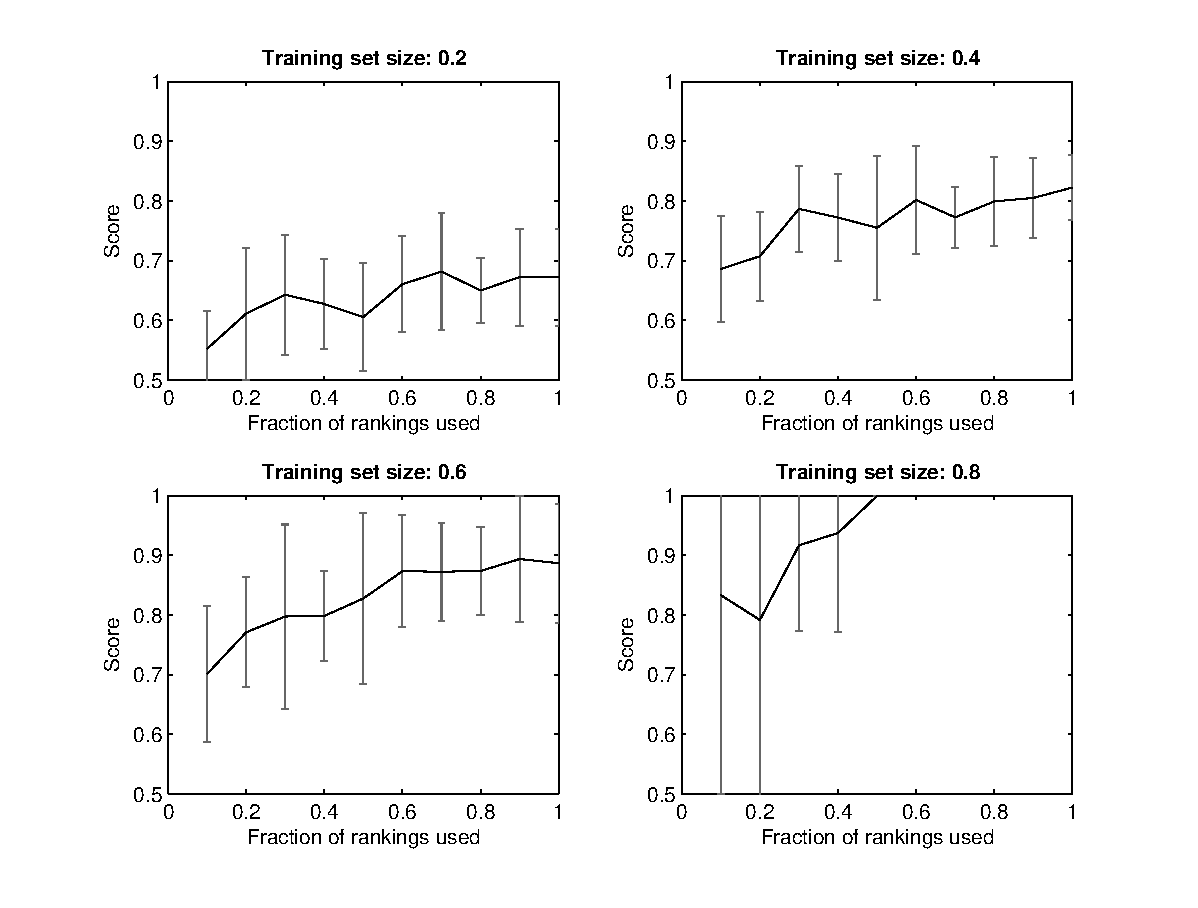
\includegraphics[width=1.1\linewidth]{rankings}
  \caption{Influence fraction of inequalities}
  \label{fig:fractie}

  \end{minipage}
  \begin{minipage}{0.5\textwidth}

      \centering
        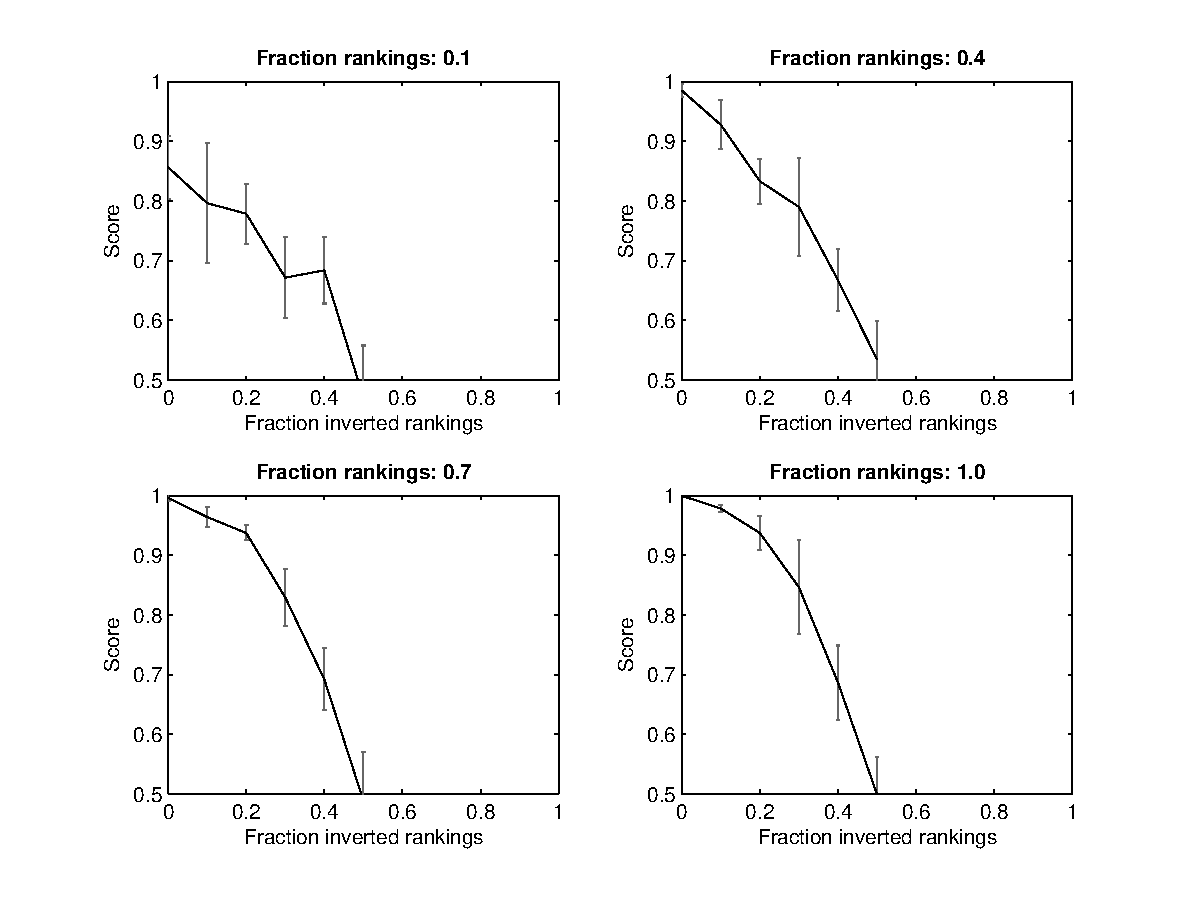
\includegraphics[width=1.1\linewidth]{noise}
      \caption{Influence of noise}
      \label{fig:ruis}

  \end{minipage}
    \end{figure}

Figure~\ref{fig:fractie} shows how the scores improve as the amount of examples and the fraction of included inequalities increases.
In all cases, more than half the pairs of examples are correctly predicted and high scores can be obtained even for small datasets.
Other experiments have shown that even for lower scores the optimization criteria are often capable of finding an optimal solution.

The underlying model can be directly expressed using the soft constraints that can be learned.
However, similar scores are obtained for models which cannot be directly modeled (e.g. the use of weighted soft constraints which are disconnected).
While there are limits to the expressibility, the learned criteria are shown to be robust with respect to the exact formulation.

The influence of noise is shown in figure~\ref{fig:ruis}.
Hereby, the second approach of testing is used, where all the examples are used as test set.
The algorithm obtains high scores despite significant levels of noise.
Figure~\ref{fig:ruis} also shows that providing more rankings improves the robustness of the algorithm, even if the relative amount of noise remains unchanged.
Using the first approach with a training set of 40\%, scores over 0.7 can be obtained for noise levels of 20\%.

  \begin{table}
    \caption{Scores for different thresholds ($t$)}
    \begin{tabularx}{\linewidth}{XXXX}
      $t = 1$ & $t = 2$ & $t = 3$ & $t = 4$ \\
      \toprule
     0.823 & 0.740 & 0.788 & 0.735 \\
     ($\pm$ 0.073)&
($\pm$ 0.078)&
($\pm$ 0.074)&
($\pm$ 0.063)
    \end{tabularx}
    \label{tbl:limiet}
  \end{table}

Finally, table~\ref{tbl:limiet} shows that increasing the threshold used for finding soft constraints does not improve the score.
This experiment used a 40\% training set and 40\% of the available rankings.
However, if the size of the problem and examples is increased, higher threshold will likely be appropriate.

\section{Conclusion}
The research in this thesis has focused on solving two problems: 1) Learning constraints; and 2) Learning optimization criteria.
Implementation for both clause learning and clausal optimization have been provided that accomplish these tasks using first order logic clauses.

The constraint learning system has been able to learn the relevant hard and soft constraints in all experiments.
As such, the first goal of this research has been accomplished.
All problems have been solved in limited time (less than a minute) and often even within a few seconds.
For each problem, only a small number of examples was given to learn from.
The system requires only a minimal amount of information from the user.
However, the system also allows for the use of expressive background knowledge.
The learned constraints are domain independent, which facilitates the construction of positive examples.

The second goal of this research, learning optimization criteria, has been accomplished as well.
Optimization criteria are discovered that enable an optimal solution to be found.
Even for small datasets and noise on the rankings, constraints are found that enable most examples to be ranked correctly.

Aside from learning formal representations automatically from examples, this research shows how these representations can be used in practice.
This also forms an important step to enable the learning of optimization criteria in an interactive setting.

\paragraph{Future work}
This research offers multiple opportunities for future work.
It would be interesting to adapt the number of variables and literals in a clause dynamically.
This could be accomplished, for example, by using negative examples.
Learned clauses must be specific enough to not cover any negative examples. 

Additionally, it would be interesting to add interactivity to the learning system for the generation of examples or rankings.
Rankings expressing that examples are equally ranked are currently ignored.
However, it could be interesting to incorporate this information into the algorithm, whenever it is provided explicitly.

As mentioned earlier, the domain independence of the clauses has several advantages.
In some cases, however, specific objects are inherently present in the problem.
The constraint learning system could be enhanced to include such global constants.

Finally, it would desirable to improve the implementation in order to tackle larger sized problems.
All the experiments were conducted with problems of limited size and the computation time increases rapidly if there are more predicates, variables and literals to be used in clauses.

\section*{Acknowledgments}
The author thanks his promoters Dr. Luc De Raedt en Dr. ir. Anton Dries.
Furthermore, he expresses his gratitude for the help provided by Bart Bogaerts, Dr. Jesse Davis, Dr. Marc Denecker and Vladimir Dzyuba.

\newpage

%
% ---- Bibliography ----
%
\bibliographystyle{aaai}
\bibliography{Bibliography}
\end{document}
